\chapter{eTrice Developer's Reference}

\section{Architecture}

The basic components of eTrice are depicted in the following diagram.

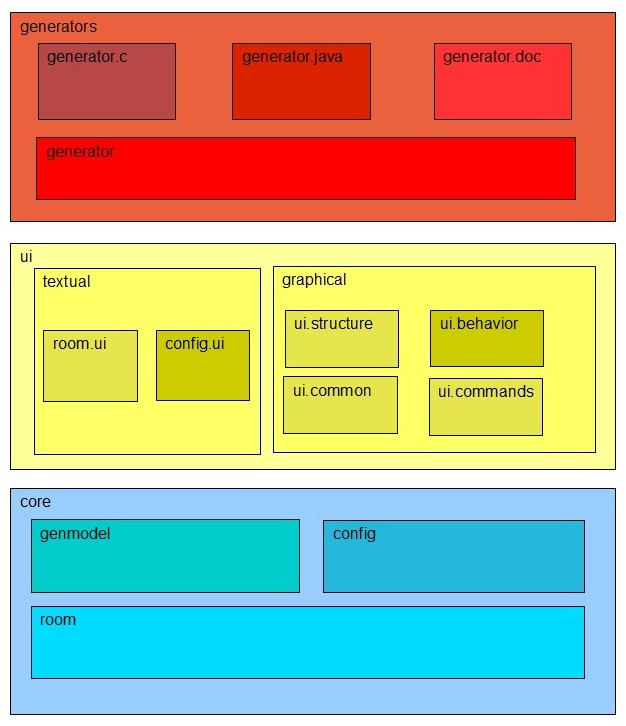
\includegraphics{images/200-components.jpg}
% !{width:50%}images/200-components.jpg!

Additional to that the eTrice project comprises runtime libraries and unit tests which are treated in subsequent sections.

\subsection{Editor and Generator Components}

\begin{itemize}
\item core

\begin{itemize}
\item core.room is an Xtext based language called Room. It consists of the plug-in \textit{org.eclipse.etrice.core.room}. Room is the basic modeling language of eTrice.
\item core.config is an Xtext based language called Config. It consists of the plug-in \textit{org.eclipse.etrice.core.config}. Config is a language designed for the data configuration of model elements. E.g. class and instance attributes can be specified.
\item core.genmodel is an EMF based aggregation layer for Room models. It consists of the plugin \textit{org.eclipse.etrice.core.genmodel}. a Room model can be transformed into a genmodel which allows easy access to implicit relations of the Room model.
\end{itemize}

\item ui
\begin{itemize}
\item textual
\begin{itemize}

\item room.ui is the ui counterpart of core.room.  It consists of the plug-in \textit{org.eclipse.etrice.core.room.ui}. This plug-in realizes IDE concepts like content assist, error markers and navigation by hyper links for the Room language.
\item config.ui is the ui counterpart of core.config.  It consists of the plug-in \textit{org.eclipse.etrice.core.config.ui}. This plug-in realizes IDE concepts like content assist, error markers and navigation by hyper links for the Config language.
\end{itemize}

\item graphical
\begin{itemize}
\item ui.common is a set of common code for the two diagram editors. It consists of the plug-in \textit{org.eclipse.etrice.ui.common}.
\item ui.commands encapsulates some commands related to the navigation between eTrice editors. It consists of the plug-in \textit{org.eclipse.etrice.ui.commands}.
\item ui.structure is the Graphiti based editor for the Actor structure. It consists of the plug-in \textit{org.eclipse.etrice.ui.structure}.
\item ui.behavior is the Graphiti based editor for the Actor behavior. It consists of the plug-in \textit{org.eclipse.etrice.ui.behavior}.
\end{itemize}
\end{itemize}

\item generators
\begin{itemize}
\item generator is a set of general classes and language independent parts of all generators. It consists of the plug-in \textit{org.eclipse.etrice.generator}.
\item generator.c is the generator for the ANSI-C target language. It consists of the plug-in \textit{org.eclipse.etrice.generator.c}.
\item generator.java is the generator for the Java target language. It consists of the plug-in \textit{org.eclipse.etrice.generator.java}.
\item generator.doc is the generator for the model documentation. It consists of the plug-in \textit{org.eclipse.etrice.generator.doc}.
\end{itemize}
\end{itemize}

\subsection{Runtimes}

Currently eTrice ships with a C and a Java runtime. The runtimes are libraries written in the target language against which the generated code is compiled.

\subsection{Unit Tests}

Most plug-ins and other parts of the code have related unit tests.

\section{Component Overview}

\subsection{Room Language Overview}

We assume that the reader is familiar with the Xtext concepts. So we concentrate on the details of our implementation that are worth to be pointed out.

\subsubsection{Model Tweaks}

The Room EMF model is inferred from the grammar. However, this powerful mechanism has to be tweaked at some places.
This is done in the \textit{/org.eclipse.etrice.core.room/src/org/eclipse/etrice/core/RoomPostprocessor.ext} which is written in the legacy Xtend language.

The following parts of the model are changed or added:
\begin{itemize}
\item the default \begin{verbatim}multiplicity\end{verbatim} of the \texttt{Port} is set to 1
\item the operation \texttt{isReplicated} is added to the \texttt{Port}
\item the default \texttt{size} of the \texttt{ActorRef} is set to 1
\item an operation \texttt{getName} is add to the \texttt{State} class
\item an operation \texttt{getName} is add to the \texttt{StateGraphItem} class
\item an operation \texttt{getGeneralProtocol} is added to the \texttt{InterfaceItem}
\end{itemize}

\subsubsection{Imports by URI Using Namespaces}

The import mechanism employed is based on URIs. This is configured for one part in the GenerateRoom.mwe2 model workflow by setting the fragments ImportURIScopingFragment and ImportUriValidator). For the other part it is configured in the Guice modules by binding
\begin{itemize}
\item \texttt{PlatformRelativeUriResolver} -- this class tries to convert the import URI into a platform relative URI. It also replaces environment variables written in \${} with their respective values.
\item \texttt{ImportedNamespaceAwareLocalScopeProvider} -- this is a standard scope provider which is aware of namespaces
\item \texttt{GlobalNonPlatformURIEditorOpener} -- this editor opener tries to convert general URIs into platform URIs because editors can only open platform URIs
\item \texttt{ImportAwareHyperlinkHelper} -- turns the URI part of an import into a navigatable hyper link
\end{itemize}

\subsubsection{Naming}

Two classes provide object names used for link resolution and for labels.
The \texttt{RoomNameProvider} provides frequently used name strings, some of them are hierarchical like State paths.
The \texttt{RoomFragmentProvider} serves a more formal purpose since it provides a link between EMF models (as used by the diagram editors) and the textual model representation used by Xtext.

\subsubsection{Helpers}

The \texttt{RoomHelpers} class provides a great deal of static methods that help retrieve frequently used information from the model.
Among many, many others
\begin{itemize}
\item \texttt{getAllEndPorts(ActorClass)} - returns a list of all end ports of an actor class including inherited ones
\item \texttt{getInheritedActionCode(Transition, ActorClass)} - get the inherited part of a transition's action code
\item \texttt{getSignature(Operation)} - returns a string representing the operation signature suited for a label
\end{itemize}

\subsubsection{Validation}

Validation is used from various places. Therefore all validation code is accumulated in the @ValidationUtil@ class. All methods are static and many of them return a Result object which contains information about the problem detected as well as object and feature as suited for most validation purposes.

\subsection{Config Language Overview}

\subsubsection{Model Tweaks}

A couple of operations are added to the ConfigModel
\begin{itemize}
\item \texttt{getActorClassConfigs}
\item \texttt{getActorInstanceConfigs}
\item \texttt{getProtocolClassConfigs}
\item \texttt{getSubSystemConfigs}
\end{itemize}

\subsubsection{Imports by URI Using Namespaces}

Imports are treated similar than in the "Room language":ImportsbyURIUsingNamespaces.

\subsubsection{Util}

A set of static utility methods can be found in the \texttt{ConfigUtil} class.

\subsection{Aggregation Layer Overview}

The eTrice Generator Model (genmodel) serves as an aggregation layer. Its purpose is to allow easy access to information which is implicitly contained in the Room model but not simple to retrieve.
Examples of this are the state machine with inherited items or a list of all triggers active at a state in the order in which they will be evaluated or the actual peer port of an end port (following bindings through relay ports).

The Generator Model is created from a list of Room models by a call of the

\begin{verbatim}createGeneratorModel(List<RoomModel>, boolean)\end{verbatim}

method of the \texttt{GeneratorModelBuilder} class.

The \texttt{Root} object of the resulting Generator Model provides chiefly two things:
\begin{itemize}
\item a tree of instances starting at each \texttt{SubSystem} with representations of each \texttt{ActorInstance} and \texttt{PortInstance}
\item for each \texttt{ActorClass} a corresponding \texttt{ExpandedActorClass} with an explicit state machine containing all inherited state graph items
\end{itemize}

\subsubsection{The Instance Model}

The instance model allows easy access to instances including their unique paths and object IDs. Also it is possible to get a list of all peer port instances for each port instance without having to bother about port and actor replication.

\subsubsection{The Expanded Actor Class}

The expanded actor class contains, as already mentioned, the complete state machine of the actor class. This considerably simplifies the task of state machine generation. Note that the generated code always contains the complete state machine of an actor. I.e. no target language inheritance is used to implement the state machine inheritance.
Furthermore the \texttt{ExpandedActorClass} gives access to
\begin{itemize}
\item \texttt{getIncomingTransitions(StateGraphNode)} -- the set of incoming transition of a \texttt{StateGraphNode} (\texttt{State}, \texttt{ChoicePoint} or \texttt{TransitionPoint})
\item \texttt{getOutgoingTransitions(StateGraphNode)} -- the set of outgoing transition of a \texttt{StateGraphNode}
\item \texttt{getActiveTriggers(State)} -- the triggers that are active in this \texttt{State} in the order they are evaluated
\end{itemize}

\subsubsection{Transition Chains}

By transition chains we denote a connected subset of the (hierarchical) state machine that starts with a transition starting at a state and continues over transitional state graph nodes (choice points and transition points) and continuation transitions until a state is reached. In general a transition chain starts at one state and ends in several states (the chain may branch in choice points).
A \texttt{TransitionChain} of a transition is retrieved by a call of \texttt{getChain(Transition)} of the \texttt{ExpandedActorClass}.
The \texttt{TransitionChain} accepts an \texttt{ITransitionChainVisitor} which is called along the chain to generate the action codes of involved transitions and the conditional statements arising from the involved choice points. 

\subsection{Generator Overview}

There is one plug-in that consists of base classes and some generic generator parts which are re-used by all language specific generators
 
\subsubsection{Base Classes and Interfaces}

We just want to mention the most important classes and interfaces.

\begin{itemize}
\item \texttt{ITranslationProvider} -- this interface is used by the @DetailCodeTranslator@ for the language dependent translation of e.g. port.message() notation in detail code
\item \texttt{AbstractGenerator} -- concrete language generators should derive from this base class
\item \texttt{DefaultTranslationProvider} -- a stub implementation of \texttt{ITranslationProvider} from which clients may derive
\item \texttt{Indexed} -- provides an indexed iterable of a given iterable
\item \texttt{GeneratorBaseModule} -- a Google Guice module that binds a couple of basic services. Concrete language generators should use a module that derives from this
\end{itemize}

\subsubsection{Generic Generator Parts}

The generic generator parts provide code generation blocks on a medium granularity. The language dependent top level generators embed those blocks in a larger context (file, class, ...). Language dependent low level constructs are provided by means of an \texttt{ILanguageExtension}. This extension and other parts of the generator be configured using Google Guice dependency injection.

\paragraph{GenericActorClassGenerator}

The \texttt{GenericActorClassGenerator} generates constants for the interface items of a actor. Those constants are used by the generated state machine.

\paragraph{GenericProtocolClassGenerator}

The \texttt{GenericProtocolClassGenerator} generates message ID constants for a protocol.

\paragraph{GenericStateMachineGenerator}

The \texttt{GenericStateMachineGenerator} generates the complete state machine implementation. The skeleton of the generated code is

\begin{itemize}
\item definition state ID constants
\item definition of transition chain constants
\item definition of trigger constants
\item entry, exit and action code methods
\item the \texttt{exitTo} method 
\item the \texttt{executeTransitionChain} method
\item the \texttt{enterHistory} method
\item the \texttt{executeInitTransition} method
\item the \texttt{receiveEvent} method
\end{itemize}

The state machine works as follows. The main entry method is the \texttt{receiveEvent} method. This is the case for both, data driven (polled) and event driven state machines. Then a number of nested switch/case statements evaluates trigger conditions and derives the transition chain that is executed. If a trigger fires then the \texttt{exitTo} method is called to execute all exit codes involved. Then the transition chain action codes are executed and the choice point conditions are evaluated in the \texttt{executeTransitionChain} method. Finally the history of the state where the chain ends is entered and all entry codes are executed by \texttt{enterHistory}.

\subsubsection{The Java Generator}

The Java generator employs the generic parts of the generator. The \texttt{JavaTranslationProvider} is very simple and only handles the case of sending a message from a distinct replicated port: \texttt{replPort[2].message()}. Other cases are handled by the base class by returning the original text.

The \texttt{DataClassGen} uses Java inheritance for the generated data classes. Otherwise it is pretty much straight forward.

The \texttt{ProtocolClassGen} generates a class for the protocol with nested static classes for regular and conjugated ports and similar for replicated ports.

The \texttt{ActorClassGen} uses Java inheritance for the generated actor classes. So ports, SAPs and attributes and detail code methods are inherited. Not inherited is the state machine implementation.

\subsubsection{The ANSI-C Generator}

The C generator translates data, protocol and actor classes into structs together with a set of methods that operate on them and receive a pointer to those data (called \texttt{self} in analogy to the implicit C++ \texttt{this} pointer).
No dynamic memory allocation is employed. All actor instances are statically initialized.
One of the design goals for the generated C code was an optimized footprint in terms of memory and performance to be able to utilize modeling with ROOM also for tiny low end micro controllers.

\subsubsection{The Documentation Generator}

The documentation generator creates documentation in LaTex format which can be converted into PDF and many other formats.
